\documentclass{article}
\usepackage{amsmath}
\usepackage{amssymb}
\usepackage{graphicx}
\title{A simple application of Shannon's entropy}
\author{Sriram Vadlamani}
\begin{document}
\maketitle
\newpage
\section{Introduction}
This document will proceed to explain a basic application of shannon's entropy on a web application such as `Netflix'.\\
We will see how a user's watch time i.e., how much of the given content (A show or a movie) has been consumed. For example,\\
A person can watch half a movie and leave it giving a 50 percent progress.\\

\section{Representation}
A user's watch time of each movie will be stored in an array as such:\\
The rows representing the various movies / shows and the columns being the various users.\\
\\
$\begin{pmatrix} 7 & 0 & 1\\ 9 & 1 & 3\\ 8 & 6 & 4 \end{pmatrix}$\\
\\
For simplicity, we will assume that the percentage completetion of content is a discrete number between 1 to 10.\\
$\forall n \in \mathbb{N}$\\
\\
\section{Entropy}
Let the probability of a user completing a given show a hundered percent i.e., in our scale, getting a 10 be `p'.\\
$P(n = 10) = p$\\
\\
Hence:\\
\\
$P(n \!= 10) = (1 - p)$\\
\\
We know, from shannon's Entropy:\\
\\
$H(P) = \sum_{x} P(x) \cdot \log_2 (1/P(x))$\\
\\
plugging in the probabilities, we should get:\\
\\
$p \cdot \log_2 (\frac{1}{p})$ $ + $ $ (1 - p) \cdot \log_2 (\frac{1}{1 - p})$\\
\\
on simplifying it, we get:\\
\\
$p \cdot \log_2 (\frac{1 - p}{p}) + \log_2 (\frac{1}{1 - p})$ bits.\\
\\
Now, if we assume the number of total users to be \textit{u}, then the total entropy would be $ u \cdot H(P)$\\
\\
\section{Visualization}
\\
If we plot the above Entropy function on a graph, this is what we get:\\
\\
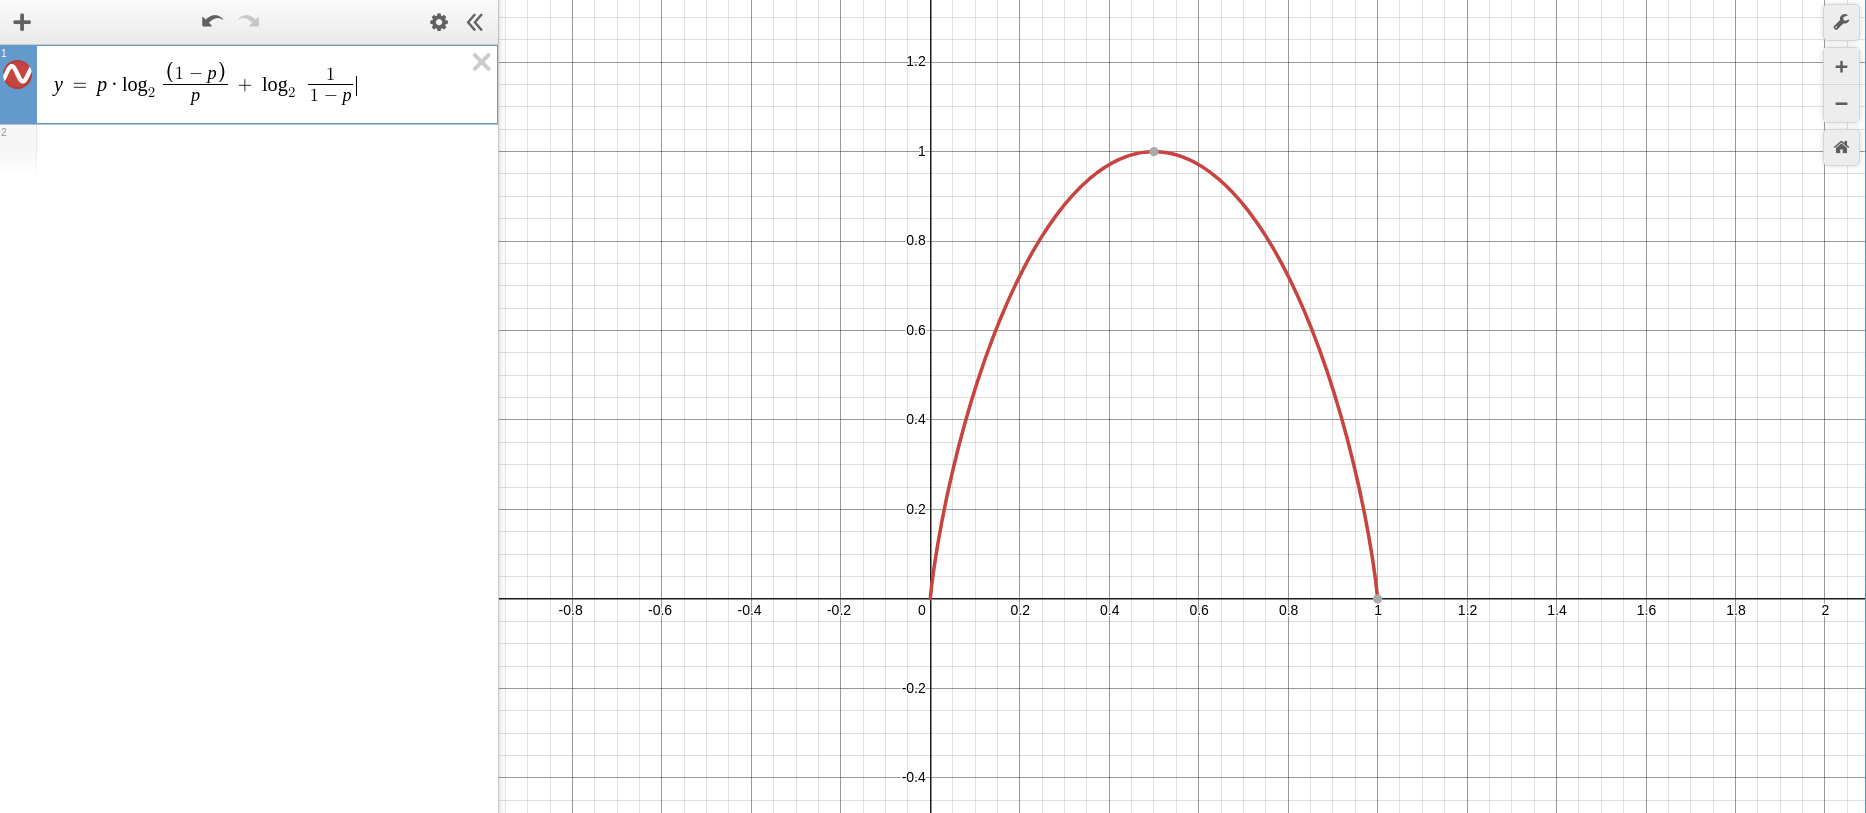
\includegraphics[width=\textwidth]{Entropy1.png}\\
\\
Now the derivative of $H(P)$ would be:\\
\\
$\frac{p^2 + (1 - p)^2}{1 - p} + \log_2 \frac{1 - p}{p}$\\
\\
Plotting a line with the hypothetical number of users, \textit{u}, we can see visually that the slope decreases as \textit{u} increases\\
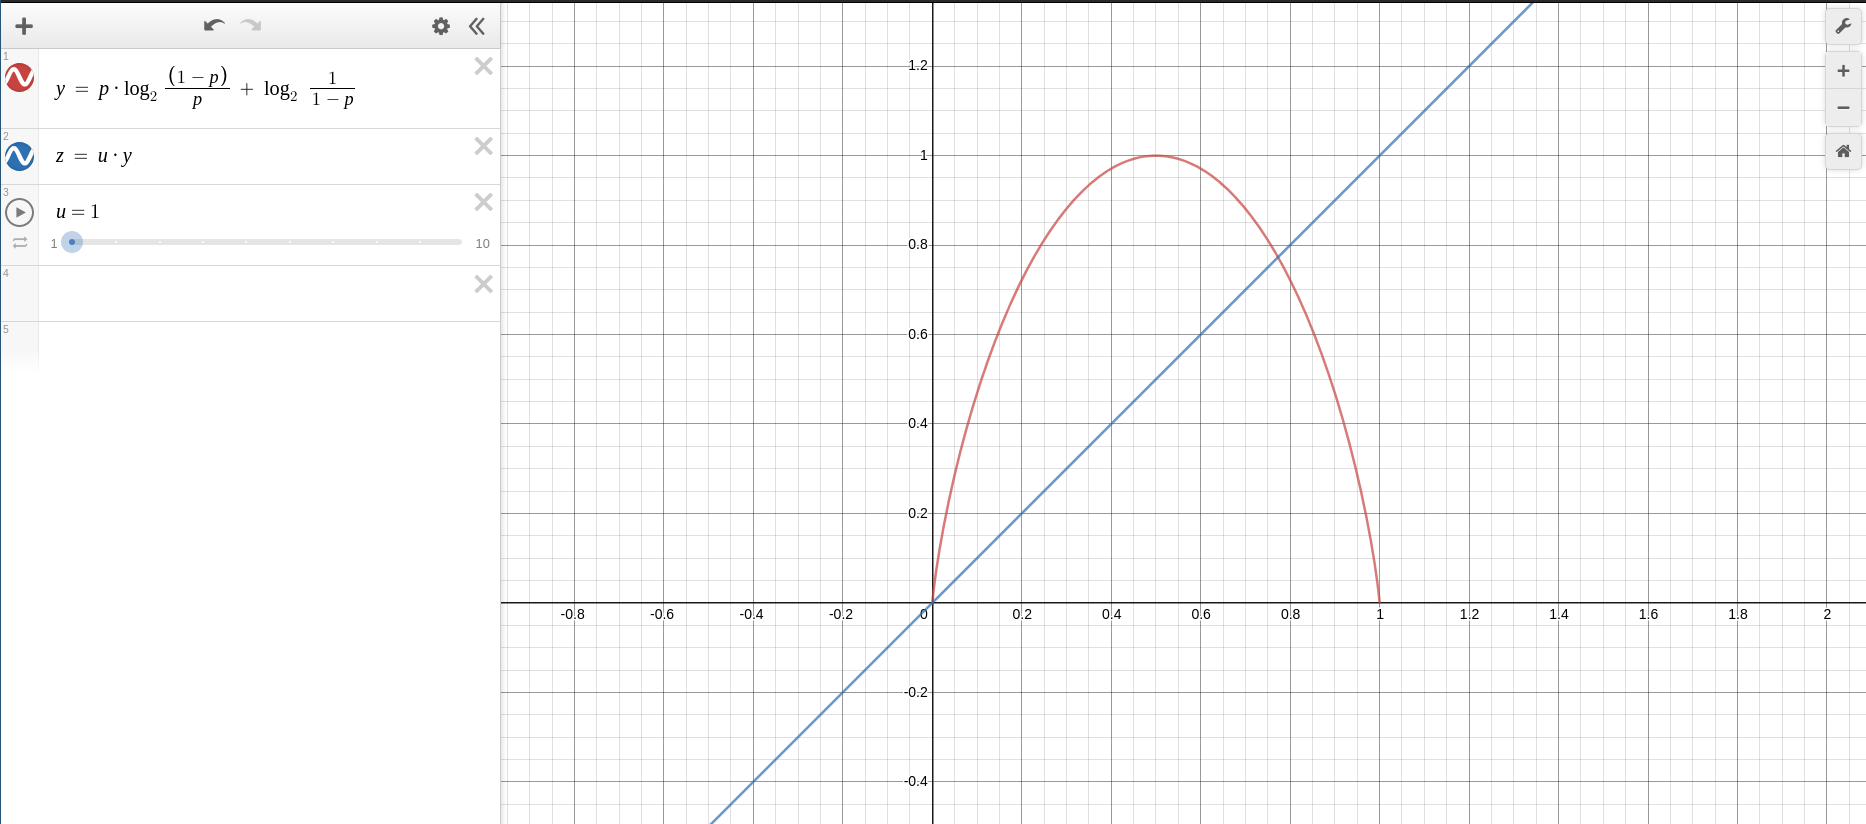
\includegraphics[width=\textwidth]{Entropy2.png}\\
\\
And when `u' = 10:\\
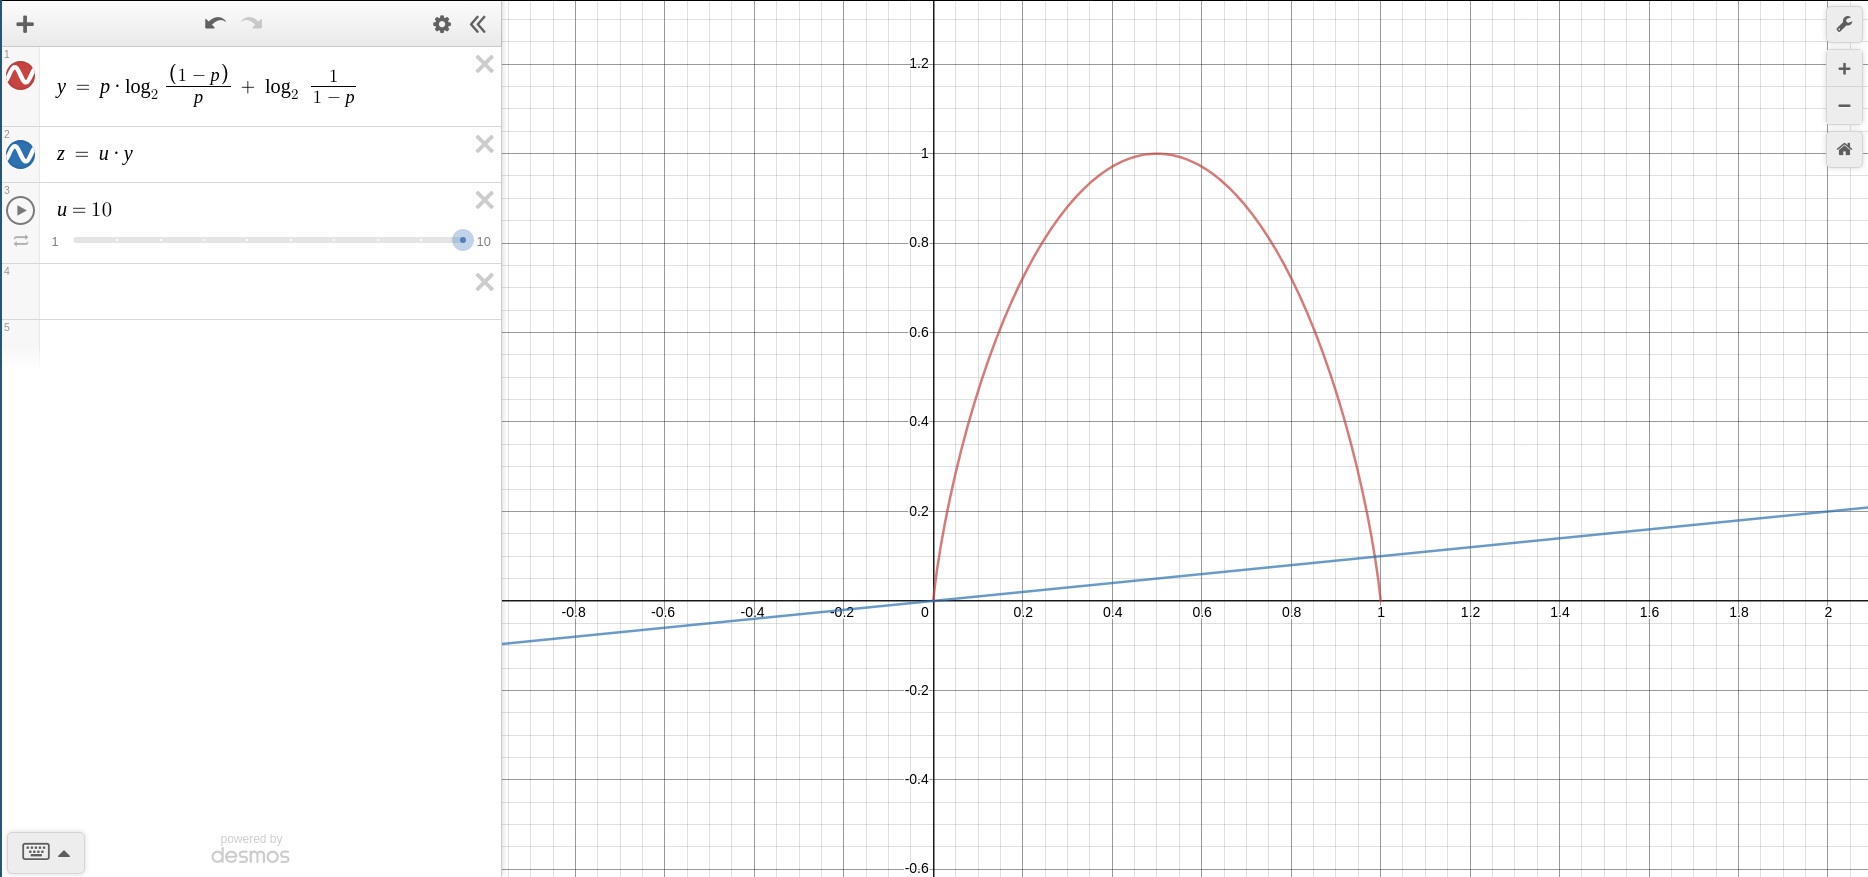
\includegraphics[width=\textwidth]{Entropy3.png}\\
\end{document}
